\section{Learning a stronger reconstruction prior}

\subsection{The change: trained 2D slices plus a trained 3D branch}

The extended solver track held the one-plate measurement model fixed and trained denoisers on reference volumes. The selected solver, t23n, uses a neuronal 2D DnCNN in all three slice orientations and adds a neuronal 3D DnCNN branch within PnP-ADMM. The 2D network has 17 layers and width 64; the 3D network has 12 layers and width 48. Both are trained with additive Gaussian corruption up to standard deviation 0.25 and learning rate 0.001. The saved runs used 30,000 iterations with batch 64 for the 2D model and 15,000 with batch 8 for the 3D model, taking about 31 minutes and 2.35 hours respectively. These are recorded run times, not a matched dimensionality benchmark. Weights are then frozen during reconstruction, and ADMM penalties are selected on held-out neuronal validation volumes.

This is not the training-agnostic operating point used in the main paper. It requires denoiser training and reference data, but does not train an end-to-end inverse network for each operator. The result tests the future direction discussed in the manuscript rather than silently replacing its original method.

\subsection{Recovery and compression range}

The following table uses the final three-noise-realisation solver block, with repeats averaged within each of eight subvolumes. Lower depth error is better.

\par\medskip\noindent\begin{minipage}{\linewidth}
\captionof{table}{Learned-prior comparison at the original detector; eight subvolumes, three noise realisations per subvolume.}
\centering
\begin{tabular}{@{}>{\raggedright\arraybackslash}p{0.227500\linewidth}@{\hspace{0.03\linewidth}}>{\raggedright\arraybackslash}p{0.227500\linewidth}@{\hspace{0.03\linewidth}}>{\raggedright\arraybackslash}p{0.227500\linewidth}@{\hspace{0.03\linewidth}}>{\raggedright\arraybackslash}p{0.227500\linewidth}@{}}\toprule
Images / compression & Generic-prior depth (\ensuremath{\mu}m) & Learned-prior depth (\ensuremath{\mu}m) & Generic / learned PSNR (dB) \\
\midrule
256 / C=1 & 0.497 & 0.346 & 31.62 / 33.20 \\
64 / C=4 & 0.538 & 0.410 & 31.16 / 32.69 \\
32 / C=8 & 0.647 & 0.503 & 30.61 / 32.11 \\
16 / C=16 & 0.689 & 0.585 & 30.15 / 31.13 \\
8 / C=32 & 0.811 & 0.820 & 29.71 / 30.00 \\
\bottomrule\end{tabular}
\end{minipage}\par\medskip


The learned 32-image result has mean depth error close to the generic-prior 256-image result. The paired difference is +0.006±0.091 \ensuremath{\mu}m across subvolumes, with foreground-SSIM change −0.018±0.056 and PSNR change +0.49±2.00 dB. This supports comparable mean depth placement at eight times fewer measurements in this test; it is not a formal equivalence test or a guarantee of identical feature recovery. The separate five-subset comparison gives 0.626\ensuremath{\rightarrow}0.476 \ensuremath{\mu}m at 32 images. These different repeat sets are kept distinct.

Gains concentrate on sparse neurite-like volumes. Dense examples show little PSNR improvement, and one large crop-level gain raises the overall mean. The initial matched comparison's median PSNR gains were approximately 1.23, 1.00 and 0.86 dB at C=1,4,8. At C=32 the learned solver does not improve depth, despite a small mean PSNR increase. Training does not remove the information limit at very small measurement counts.

\subsection{Leakage screen and controls}

Because the stored references are crops of one parent stack without saved crop coordinates, training overlap was checked by an FFT shift/correlation screen. It excluded 141 of 1,013 candidate crops; 16 cleared crops were held out for validation, leaving 856 for training. A stricter re-screen found one genuine overlap just below the original volume threshold: training crop 1015 shares 1.99\% with test crop p576. Excluding p576 left the learned-prior conclusion intact. This is a documented residual overlap, not a claim of a perfect leakage screen.

A vasculature-trained 2D/3D prior, tuned on the same neuronal validation volumes, gave full-measurement depth error 0.355 \ensuremath{\mu}m on the neuronal test set, close to the neuronal prior's 0.346 \ensuremath{\mu}m and below the generic prior's 0.497 \ensuremath{\mu}m. This supports a benefit beyond simply reproducing the neuronal training collection, although it is not an independent biological validation.

On synthetic beads, the neuronal prior produced zero false detections in the tested cases and Jaccard index 1.00. Depth error improved from 0.135 to 0.065 \ensuremath{\mu}m at full measurements and from 0.204 to 0.110 \ensuremath{\mu}m at 32 images. PSNR fell because the learned prior altered bead intensity profiles. Thus accurate localisation and intensity fidelity can move in opposite directions; these bead controls differ from the main paper's sparsity-prior bead results.

With an in-focus DMD, the learned solver still gave 1.226 \ensuremath{\mu}m depth error versus 0.346 \ensuremath{\mu}m with the phase plate at full measurements. The prior improved reconstruction but did not replace missing depth discrimination. A paraxial phase-plate control gave 0.354 \ensuremath{\mu}m with the learned solver, close to the reference angular-spectrum model.

\textbf{Conclusion:} learned volumetric priors are a useful compression lever in this collection, especially when combined with 2D slice priors. Their benefits depend on object structure and must be distinguished from the information supplied by the acquisition.

Evidence: D22; {\small\texttt{solver\_\allowbreak{}learned/\allowbreak{}README.\allowbreak{}md}}, overlap-screen files and test rows; final master-table solver and encoder-control blocks.


\begin{figure}[htbp]
\centering
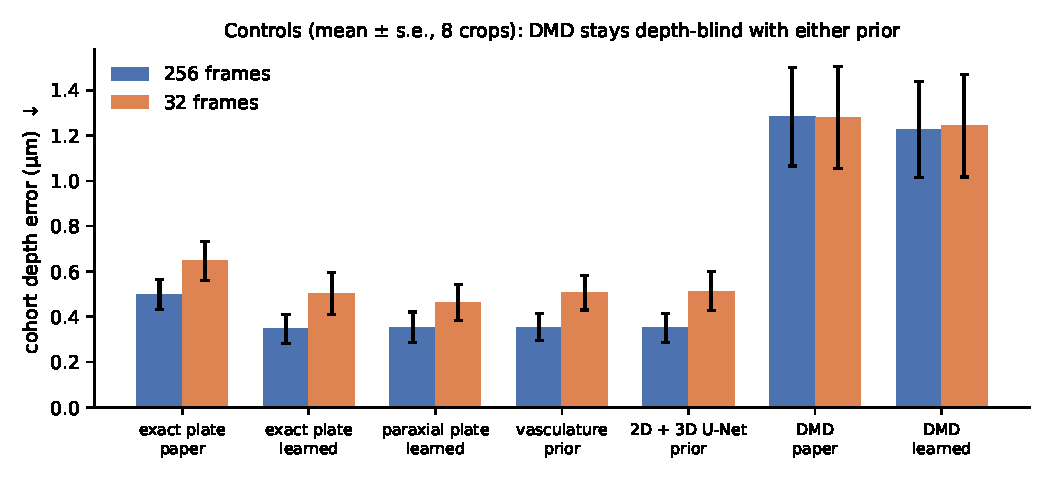
\includegraphics[width=\linewidth,height=0.48\textheight,keepaspectratio]{figures/prior_controls.pdf}
\caption{Encoder and prior controls. The same learned reconstruction remains depth-ambiguous with the in-focus DMD; the paraxial plate and vasculature-trained prior retain the phase-plate benefit. Bars compare 256 and 32 images; error bars are standard errors across eight test subvolumes. Original final-package plot.}
\label{exp:fig_controls}
\end{figure}
\FloatBarrier
